\documentclass[11pt]{article}
%==============================================================================
% Basic Packages {{{ 
%==============================================================================
\usepackage{mathpazo}
\usepackage[top=2cm, bottom=3.5cm, left=2.5cm, right=2.5cm]{geometry}

\usepackage{graphicx}                               %insert images
\usepackage{verbatim}                               %include txt files
\usepackage{cite}

\usepackage{amsmath,amsfonts,amssymb,amsthm}        %basic math support
\usepackage{tikz-cd}                                %draw commutative diagrams
\usetikzlibrary{graphs}                             %draw graphs with tikz
\usepackage{bussproofs}                             %proof trees
\usepackage{algorithm,algpseudocode}                %pseudocode algorithms

% }}}

%==============================================================================
% Page Setup {{{
%==============================================================================
\author{Eli Rosenthal \and Will Kochanski}
\date{}

\setlength{\parindent}{0pt}
% }}}

%==============================================================================
% Macros {{{
%==============================================================================
\newcommand{\img}[1]{\begin{center}
    \includegraphics[width=0.8\textwidth]{#1}
\end{center}}

\newenvironment{bprooftree}
    {\leavevmode\hbox\bgroup}
    {\DisplayProof\egroup}

\newcommand{\ir}[1]{\textnormal{\sc#1}}
\newcommand{\tx}[1]{\textnormal{#1}}
\newcommand{\arr}{\rightarrow}

\newcommand{\R}{\mathbb{R}}


\newtheorem{Thm}{Theorem}
\newtheorem{Lem}{Lemma}
\newtheorem{Cor}{Corollary}
% }}}

\title{Paper Summary: An Elementary Proof of a Theorem of Johnson and Lindenstrauss}
\begin{document}
%==============================================================================
% Begin Document
%==============================================================================
\maketitle
\section{Introduction}
In data analysis we often want to produce summary information to concisely describe \textit{static} and \textit{global} properties of a large data set. However, for some operations most if not all of the structure in the original data is needed; consider removing outliers from a dataset, or finding the nearest neighbor to a given point. Many queries like this are either \textit{dynamic} and change the shape of the data, or \textit{local} and need access to only part of the data. To perform these operations efficiently we need to reduce the size of our representation, while preserving the structure of our data, an example of this is \textbf{Dimensionality Reduction}.

\section{Dealing with High Dimensions}
Many data sets, such as a collection of photographs, can be described formally as a set of points in euclidean space; with each coordinate storing the intensity of a given pixel. In low dimensions we can often differentiate between datasets which behave well under projection, and datasets which do not. Consider the two figures below:

\begin{center}
    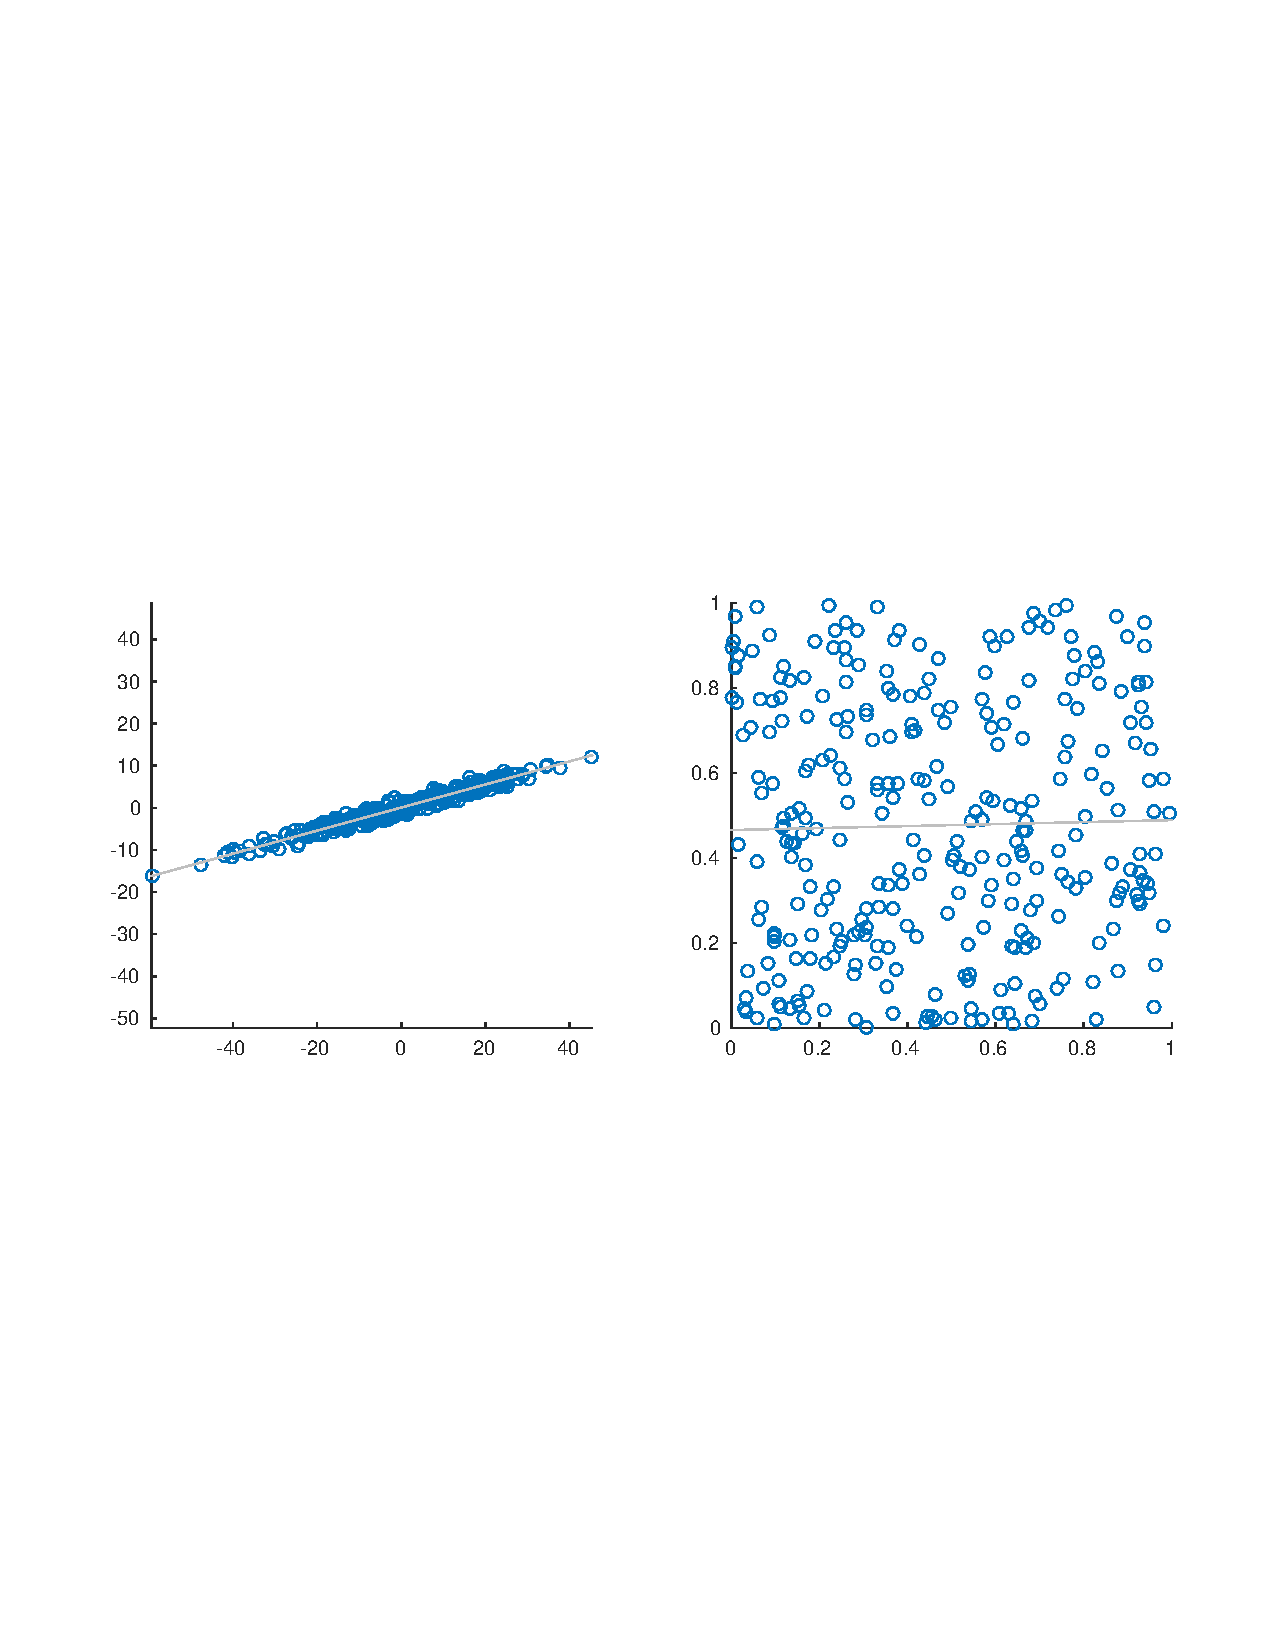
\includegraphics[trim=0 280 0 280, clip, width=\textwidth]{2dplots.pdf}
\end{center}

The set on the left can be represented almost faithfully by projecting onto the one dimensional space represented by the central line, relative distances will be roughly preserved with the largest deviation near the center of the bounding ellipse. On the right, however, there is no good line to project onto; no matter what we choose we will have to collapse many disperse points to the same neighborhood. 

The surprising result of Johnson and Lindenstrauss \cite{oldpaper} is that in high enough dimensions there is no such distinction. In fact, by projecting onto a \textit{random} subspace we can reduce the dimension without significantly distorting pairwise distance.

\section{The Johnson Lindenstrauss Theorem}
Formally we are interested in the distortion of \textit{pairwise distance}. If the map $f : \R^d \arr \R^k$ is a projection from a high dimensional space $\R^d$ to a space of lower dimension $\R^k$ then for any two points $u, v \in \R^d$ the ratio
\[ \frac{\| f(u) - f(v) \|^2}{\| u - v \|^2} \]
Measures how the distance between the two points changes under the projection. By capturing pairwise distances we can imagine preserving a rigid skeleton of our data from which further information such as the angles between points can be deduced. Moreover, distortion is indepedent of the absolute scale and position of the data, which allows both large and small features such as ``clumps'' to be preserved. The main theorem presented in this paper \cite{mainpaper} is that we can choose $k$ large enough such that \textit{no} pairwise distance will be distored by more than a constant factor.

\begin{Thm}
  For any $0 \leq \epsilon \leq 1$, and any integer $n$, let $k$ be a positive
  integer such that
  \[ 
    k \geq 4(\epsilon^2/2 - \epsilon^3/3)^{-1} \ln n 
  \]
  Then for any set of $n$ points $V \subseteq \R^d$, there exists a map
  $f:\R^d \arr \R^k$ such that for all $u, v \in V$
  \[
    (1-\epsilon)\|u - v\|^2 \leq \| f(u) - f(v) \|^2 \leq (1+\epsilon) \| u - v \|^2 
  \]
  Furthermore, this map can be found in randomized polynomial time.
\end{Thm}

Here $\epsilon$ is a tolerance parameter which captures how much distortion we are willing to accept for any pair of points. If we fix $\epsilon = 0.1$ then this theorem says that we can represent a dataset of $n$ points in about $1000 \ln n$ dimensions with no more than 10\% distortion on any pair. At first it may seem surprising that the target dimension $k$ is bounded by $n$ and \textbf{not} the source dimension $d$. One view is that since we only concerned with \textit{relative} distances between points we can always rotate our data to fit in $n$ dimensions, so all we need is to produce a map $\R^n \arr \R^k$. A more subtle perspective comes from answering the question: What does it mean that this map can be found in randomized polynomial time?

This paper presents a simple \textit{randomized} algorithm: choose a random projection and check whether the distortion is bounded, keep trying until it works. Using a union bound the probability of failure is proportional to the number of pairwise distances, so in order to bound this probability we give constraints in terms of $n$.

\section{Section}


The statement of the theorem is rather interesting: the bounds we get on
distortion are in terms of $\epsilon$ which is in turn bounded in terms of $k$
and $n$ but not $d$. This is the first clue that we are dealing with some sort
of random algorithm. This algorithm is roughly the following: pick a unit vector
of length $k$ from some Gaussian distribution. Then pick $n-1$ additional random
unit vectors that are orthogonal to this first vector: left-multiplying a vector
in $n$ dimensions by this new matrix yields a point in $\mathbb{R}^k$.

-- Contextualization of variables
-- Intuition, when projected length is tightly concentrated around mean

-- Intuition for a random projection
-- rotational invariance, linear scaling, allows us to analyse a random vector.

\subsection{Sampling from the Unit Sphere}
It turns out that sampling a random unit vector from the unit sphere is not exactly obvious. We have provided a few ways (Figure~\ref{fig:spheres}) that one might sample from the unit sphere $S^d$, and some obvious ways aren't uniform!

\begin{figure}
  \begin{center}
    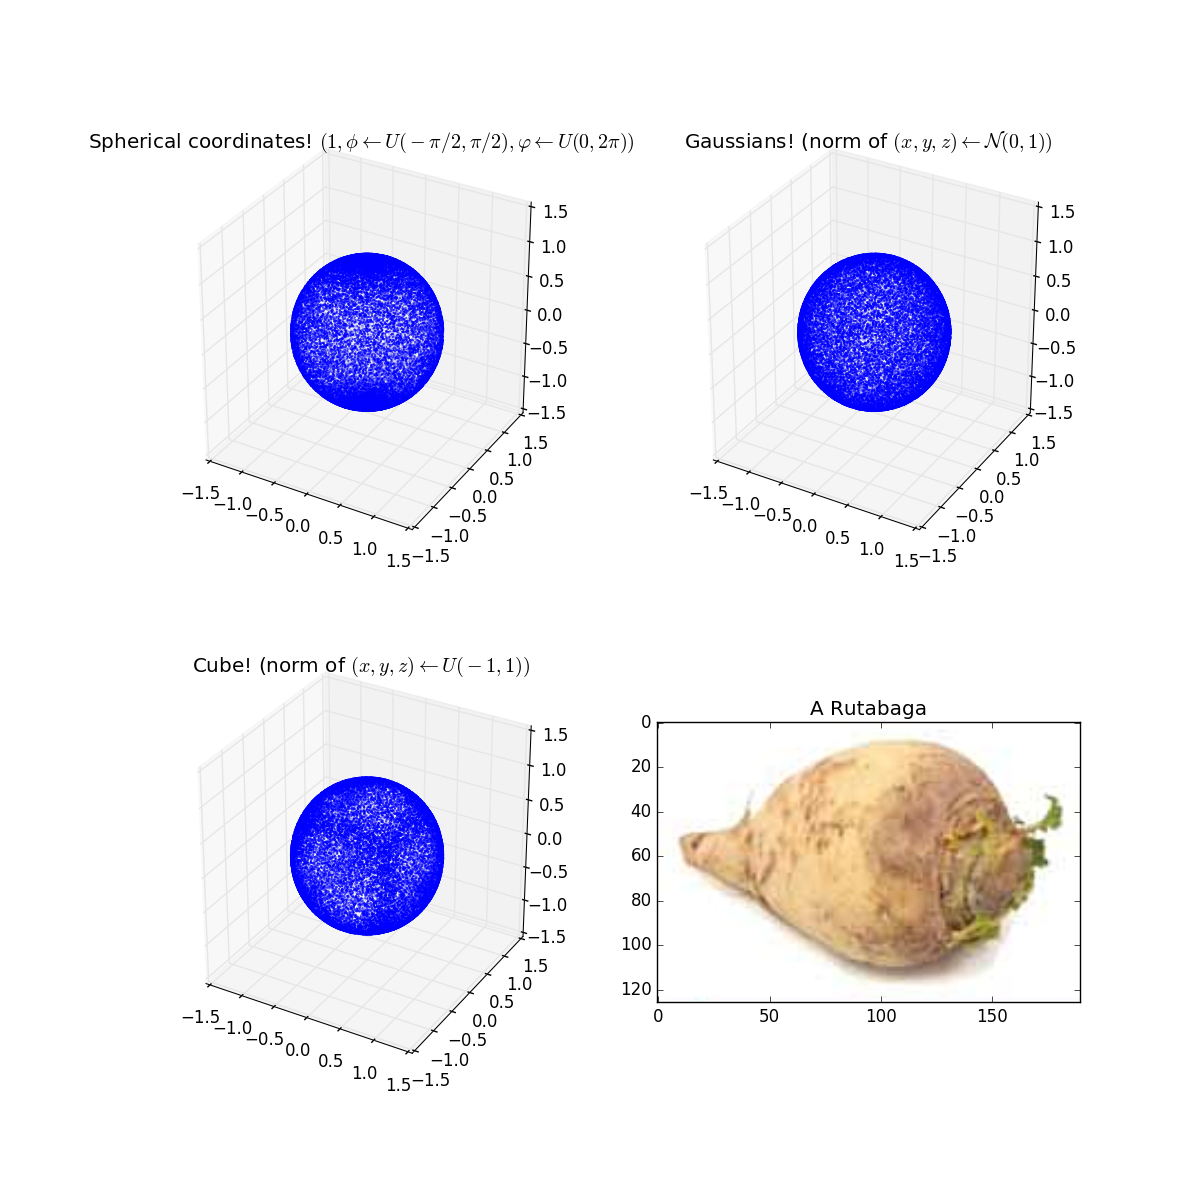
\includegraphics[width=0.9\linewidth]{spheres.png}
  \end{center}

  \caption{Randomly sampling a sphere with spherical coordinates, cubical
    coordinates, and a normal distribution. Note that only a normal distribution
    is free of spots with greater and lower density}
  \label{fig:spheres}
\end{figure}

An important insight here is that we do not have to sample from the sphere directly, instead we can sample from ther larger space of $\R^d$ and normalize the result to obtain a point on the sphere. All we need is a rotationally symmetric distribution, so that the result of normalization will be uniform. As it happens this is easy to provide, if each coordinate $X_i$ is sampled independently from the standard normal distribution then we can write the joint pdf
\[ p(X_1,X_2,...,X_d) = \prod_{i} p(X_i) = c \times \exp(\frac{1}{2} (X_1^2 + X_2^2 + ... X_d^2)) \]
For some constant $c$. Since this can be re-written as a function of the length of $(X_1,X_2,...,X_d)$ the distribution must be symmetric. This also has the advantage that each component is sampled identically and independently at random, allowing us to use Chernoff bounds to analyse the resulting vector (see Figure~\ref{fig:bounds}).

    \begin{figure}[H]
      So you're sampling from some distribution, and you want to know how fast
      you converge to ground truth.

      \begin{tabular}{lll}
        What do you know? & Distribution & Tail bound\\
        \hline
        I know something about the mean..  & Markov! & Linear \\
        I know something about the variance..  & Chebyshev! & quadratic/polynomial\\
        My samples are i.i.d.  & Chernoff! & \emph{Exponential}\\
        \hline
      \end{tabular}
      \caption{Sampling cheat sheet}
      \label{fig:bounds}
    \end{figure}


\bibliography{refs}{}
\bibliographystyle{plain}

\end{document}
